\documentclass{article}
\usepackage{graphicx}
\usepackage{amsmath}
\PassOptionsToPackage{svgnames}{xcolor}
\usepackage{tcolorbox}
\usepackage{xcolor}
\usepackage{lipsum}
\usepackage{verbatim}
\tcbuselibrary{skins,breakable}
\usetikzlibrary{shadings,shadows}
\usepackage{float}
\usepackage{hyperref}
\usepackage[a4paper]{geometry}
\usepackage{listings}
\usepackage{titlesec}
\usepackage{amssymb}
\usepackage[T1]{fontenc}
\usepackage{multirow} % for Tables
\usepackage{fancyvrb} % for "\Verb" macro
\VerbatimFootnotes % enable use of \Verb in footnotes
\usepackage{listings}
\lstset{basicstyle=\ttfamily,
  showstringspaces=false,
  commentstyle=\color{green},
  keywordstyle=\color{blue}
}

\setcounter{secnumdepth}{4}
\titleformat{\paragraph}
{\normalfont\normalsize\bfseries}{\theparagraph}{1em}{}
\titlespacing*{\paragraph}
{0pt}{3.25ex plus 1ex minus .2ex}{1.5ex plus .2ex}

\title{\textbf{Terraform}}
\author{Alejandro Campos}
\date{June, 2024}

\setlength{\parindent}{0ex}
\setlength{\parskip}{6pt}
\geometry{top=2.5cm, bottom=3cm,left=3cm, right=3cm}
\hypersetup{
    colorlinks=true,
    linkcolor=black,
    filecolor=magenta,
    urlcolor=blue,
}

\definecolor{codegreen}{rgb}{0,0.6,0}
\definecolor{codegray}{rgb}{0.5,0.5,0.5}
\definecolor{codepurple}{rgb}{0.58,0,0.82}
\definecolor{backcolour}{rgb}{0.95,0.95,0.92}

\newenvironment{blocktemplate}[1]{%
    \tcolorbox[beamer,%
    noparskip,breakable,
    colframe=Blue,%
    colbacklower=LimeGreen!75!LightGreen,%
    title=#1]}%
    {\endtcolorbox}

\newenvironment{blocktemplateI}[1]{%
    \tcolorbox[beamer,%
    noparskip,breakable,
    colframe=Violet,%
    colbacklower=Black,%
    title=#1]}%
    {\endtcolorbox}

\newenvironment{blocktemplateII}[1]{%
    \tcolorbox[beamer,%
    noparskip,breakable,
    colframe=Green,%
    colbacklower=LimeGreen!75!LightGreen,%
    title=#1]}%
    {\endtcolorbox}

\newenvironment{blocktemplateIII}[1]{%
    \tcolorbox[beamer,%
    noparskip,breakable,
    ,colframe=Red,%
    colbacklower=LimeGreen!75!LightGreen,%
    title=#1]}%
    {\endtcolorbox}

\newtcolorbox{mybasecolorbox}[1][]{%
  colback=gray!25, colframe=gray!25,
  coltitle=black,
  width=(\linewidth-20pt)}

\newenvironment{codetemplate}[1][]{%
  \mybasecolorbox[#1]
  \itshape
}{%
  \endmybasecolorbox
}

\begin{document}
\maketitle
\newpage
\tableofcontents
\newpage

%====================================================================================================
\newpage
\section{Introduction}

\subsection{What is NGINX?}

NGINX is an open source web server written in C and can also be used as a reverse proxy and a load balancer. It serves the web content (static or dynamic) listening on an HTTP endpoint and understand how to talk this HTTP protocol.

As a \textbf{reverse proxy}, you can make NGINX face the internet getting the requests and then, internally it moves these requests across your back ends appropiately, it also can morph the request, authenticate the request, change the request, etc. It also can check if the back-end is down to not redirect traffic to this back-end. So in summary, reverse can provide:
\begin{itemize}
    \item \textbf{Load Balancing:} balance the requests between \textit{n} instances of back-end.
    \item \textbf{Back-end Routing:} redirect the traffic to one back-end or another depending on: the path they use, the domain, etc.
    \item \textbf{Cache:} cache requests that are repetitive directly on the NGINX, to avoid ask the back-end for some of the requests. Minimizing the latency and resource consumtion.
    \item \textbf{Firewall:} filter traffic, number of requests, etc. To avoid malicious usage of the back-ends.
\end{itemize}

\subsection{Why do we need NGINX?}

Imagine that we have our web application running without NGINX serving HTTPS. We should have:

\begin{itemize}
    \item Physical Server or VM running on port 443 the service or docker container with the web content.
    \item Certificate installed and configured on the service or docker container.
    \item Router (public IP) with the port 443 opened to the World and forwarded to the same port on physical server.
\end{itemize}

What would happen if we want to grow up this infrastructure, we will need new servers, open new ports on the router, give the new ports to all the customers... It will be a mess, and if we have HTTPS what would you do? Share the certificate between all the new servers? It is dificult to handle. And what would happen if one of the machine is down? You would need to tell the client: hey, don't go to this port because it is down. It is a lot of work, isn't it?

That's why we introduce an extra layer as \textbf{reverse-proxy}, NGINX.

\begin{itemize}
    \item HTTPS it's only configured from NGINX out, it uses HTTP to communicate withe the back-ends or you can as well enable more security and communicate using SSL but without having the web certificate in all the back-ends. So the web certificate just need to be configured on NGINX.
    \item NGINX completely hide back-ends, so clients just talk with NGINX, and it's NGINX who decides to which back-end send the requests, how, do it or not do it, etc.
    \item NGINX will load balance the request (by default using round-robin), and if one back-end is not alive it will not send requests to it.
\end{itemize}

\begin{figure}[H]
    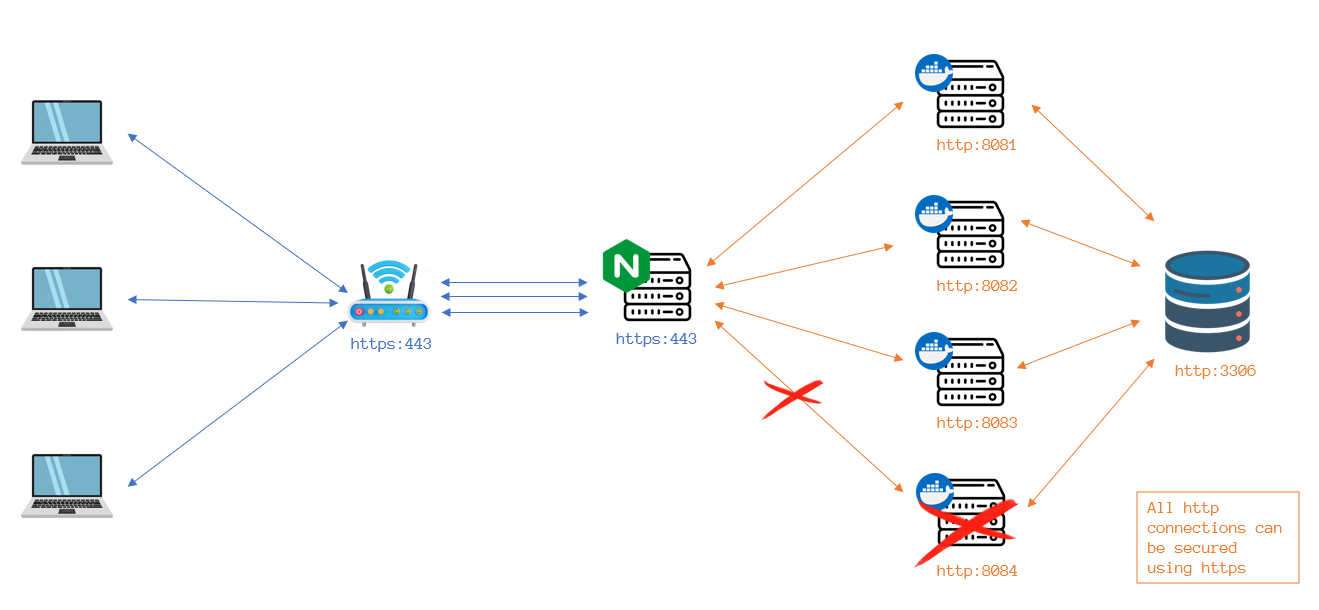
\includegraphics[width=\textwidth]{pictures/scheme_nginx.png}
    \centering
\end{figure}

\begin{blocktemplateII}{Note}
Round-robin load balancing is a method used to distribute network traffic across multiple servers. It ensures that no single server is overwhelmed with too many requests. Here’s how it works:
\\\\
\textbf{Request Distribution:} Incoming requests from clients are distributed to a pool of servers in a cyclic order.
Each server in the pool gets an equal number of requests over time.
\\\\
\textbf{Sequential Assignment:} The load balancer maintains a list of servers.
The first incoming request is sent to the first server, the second request to the second server, and so on.
Once the load balancer reaches the end of the list, it cycles back to the beginning.
\\\\
\textbf{Cycle Repeat:} This process repeats continuously, ensuring that each server receives traffic in a round-robin fashion.
For example, if there are three servers (A, B, C), the request distribution would follow the pattern: A, B, C, A, B, C, and so on.
\\\\
\textbf{Cons:} 
\begin{itemize}
    \item \underline{Not Load-Aware:} Standard round-robin does not account for the current load on each server, potentially leading to inefficiencies.
    \item \underline{Performance Variations:} If servers have different performance capabilities, a plain round-robin approach might not utilize the servers optimally.
    \item \underline{Session Persistence:} Does not inherently support session persistence (also known as sticky sessions), where a client's requests need to be handled by the same server.
\end{itemize}
\end{blocktemplateII}

The clients have no idea that their requests are going to one of the back-end servers, they just see the NGINX. In the same way, the back-end servers don't know the originating client of the requests they are answering, they know NGINX makes the request.

\begin{blocktemplateI}{Note}
Just to clarify, from now, we are going to talk about:
\begin{itemize}
    \item \textbf{NGINX Front-end:} communication between NGINX and the clients.
    \item \textbf{NGINX Back-end:} communication between NGINX and the servers (back-ends).
\end{itemize}
\end{blocktemplateI}

You can configure your NGINX to perform at Layer 4, Layer 7 or both at the same time through the configuration NGINX file.

\subsection{NGINX Layer 4 vs Layer 7 Proxing}
Let's make a refresh on OSI Layers:

\subsubsection{Layer 4 - Transport Layer}

Transmits data using transmission protocols (like UPD and TCP). So information we have on Layer 4:
\begin{itemize}
    \item Source IP and source Port (plain text information, never encrypted).
    \item Destination IP and destination Port (plain text information, never encrypted).
    \item Packet inspection: SYN (to stablish conneciton), TSL (to retrieve some data).
\end{itemize}

It is really useful when NGINX doesn't really understand the protocol, like for example a Postgres db protocol or MySQL. NGINX does not know how to terminate it, read it, parse it, turn around and talk to a backend that understand it.

\textbf{NGINX on Layer 4:}
\begin{itemize}
    \item Block connections from source IPs or source Ports.
    \item Block connections to destination IPs or destination Ports.
    \item Raise events based on Layer 4 data retrieved.
\end{itemize}

\subsubsection{Layer 7 - Application Layer}
Human-computer interaction layer, where applications can access the network services. All application data use to be encrypted, so the reverse proxy \textbf{decrytps} all this data.

\textbf{NGINX on Layer 7:}
\begin{itemize}
    \item Type of connection: HTTP, HTTPS, gRPC, etc.
    \item Filter, modify, redirect based on context.
    \item Know which pages clients are visiting, the headers of the requests, the cookies of the requests, the cookies of the navigator, etc.
\end{itemize}

It is really useful when NGINX understand the protocol, like for example HTTP or HTTPS, because it enables NGINX to redirect traffic, parse, modify, rewrite or add more headers, cache, etc.

\subsection{TLS Termination vs TLS Passthrough}

\subsubsection{Introduction}

\textbf{TLS (Transport Layer Security)} is a way to establish end-to-end encryption between one another, every time you use HTTPS your are using TLS. It uses a symmetric encryption for communication (client and server has the same key).

So the question is mandatory, how can I share the key in plain text? TLS uses \textbf{Asymmetric Encription} to exchange the symmetric key.

The reason for not do it all using Asymmetric Encryption is because it is very slow compared to Symmetric Encryption, so it will increase a lot the latency in all the connections, and we don't want that.

\subsubsection{Certificates}
How can you guarantee as server or client who are you talking to? There is no method of authentication, so anyone in the middle can just stop the key exchange and then reply back and sey: hey I'm the server or the client. And then intercept all the connections, decrypt them, and encrypt them again using its own key, performing a terminaton of TLS. It is commonly named as \textbf{man in the middle}.

How can we actually identify that you are talking with the right endpoint you want to talk? Using Certificates, that nobody else except the servers has. So, the server during the handshake of the TLS, will reply back with its own certificate, signed by a Certificate Authority (or certbot XD) demonstrating that he actually is which it says it is. 

As well as server, client can be authenticate, and that's when we name the connection as \textbf{MTLS}

\subsubsection{NGINX doing TLS Termination}
NGINX can use HTTPS (TLS) meanwhile the back-ends not (you can choose to secure as well this connection). So NGINX does the same as \textbf{man in the middle}, it \textbf{terminates} the TLS connection, it \textbf{decrypts} all the data and send to the back-ends unencrypted (or encrypted if you enable the feature). 

NGINX does this because he is the one which negotiates the key exchange with the clients and servers. So anyone sniffing traffic between the client and the NGINX won't see anything, because it is all encrypted, but if he is in the middle of the NGINX connections with the back-ends, he will see everything. But... If you have your infrastructure on a private network. Who would be sitting on your network? 

So for cloud resources it is recommended to encrypt both sides (NGINX front-end connections and NGINX back-end connections). So in that case, NGINX will make the key exchange with the back-ends and encrypt the data again for them.

So for doing all of that, NGINX should have its own certificate with private and public keys configured inside.

\subsubsection{NGINX doing TLS Passthrough}
As well, you can configure NGINX to not TLS Terminate the connections, to don't act as man in the middle. So NGINX can just pipe everything through itself and send it to the backend with all the properties of load-balancing and that stuff, but without decrypt and encrypt anything. NGINX then will just stream the packets directly to the backends. And then, will be responsible of the back-ends to handle with certificates and keys.

The bad thing on this configuration is that NGINX cannot see anything regarding \textbf{Layer 7}, because the encryption is end-to-end. So NGINX cannot take any decition based on this data, just act as Layer 4 proxy, deciding what to do with the traffic just based on IP's and Ports.

\subsection{NGINX Internal Architecture}






























\end{document}